\documentclass[11pt]{article}
\usepackage[margin=1in]{geometry}
\usepackage[T1]{fontenc}
\usepackage{lmodern}
\usepackage{microtype}
\usepackage{amsmath}
\usepackage{graphicx}
\usepackage{booktabs}
\usepackage{tikz}
\usetikzlibrary{arrows.meta,positioning,patterns}
\usepackage[hidelinks]{hyperref}
\usepackage{xcolor}
% generated by make_numbers.py from RESULTS.md
\expandafter\def\csname v@live.errors\endcsname{2}
\expandafter\def\csname v@live.extensionOriginRequestsDuringBrowsing\endcsname{0}
\expandafter\def\csname v@live.loads\endcsname{58}
\expandafter\def\csname v@live.minutes\endcsname{10}
\expandafter\def\csname v@pb.default.med\endcsname{2375}
\expandafter\def\csname v@pb.default.n\endcsname{8}
\expandafter\def\csname v@pb.default.pre\endcsname{0}
\expandafter\def\csname v@pb.default.spec\endcsname{1}
\expandafter\def\csname v@pb.errors\endcsname{169}
\expandafter\def\csname v@pb.extension.med\endcsname{575}
\expandafter\def\csname v@pb.extension.n\endcsname{7}
\expandafter\def\csname v@pb.extension.pre\endcsname{4}
\expandafter\def\csname v@pb.extension.spec\endcsname{9}
\expandafter\def\csname v@pb.instantpage.med\endcsname{1622}
\expandafter\def\csname v@pb.instantpage.n\endcsname{8}
\expandafter\def\csname v@pb.instantpage.pre\endcsname{1}
\expandafter\def\csname v@pb.instantpage.spec\endcsname{4}
\expandafter\def\csname v@pb.quicklink.med\endcsname{1584}
\expandafter\def\csname v@pb.quicklink.n\endcsname{8}
\expandafter\def\csname v@pb.quicklink.pre\endcsname{4}
\expandafter\def\csname v@pb.quicklink.spec\endcsname{87}
\expandafter\def\csname v@r0.clarknet_aug28.ci.bm.hi\endcsname{-2.03}
\expandafter\def\csname v@r0.clarknet_aug28.ci.bm.lo\endcsname{-2.32}
\expandafter\def\csname v@r0.clarknet_aug28.ci.bp.hi\endcsname{-0.26}
\expandafter\def\csname v@r0.clarknet_aug28.ci.bp.lo\endcsname{-0.28}
\expandafter\def\csname v@r0.clarknet_aug28.ci.hm.hi\endcsname{0.73}
\expandafter\def\csname v@r0.clarknet_aug28.ci.hm.lo\endcsname{0.33}
\expandafter\def\csname v@r0.clarknet_aug28.ci.hp.hi\endcsname{0.90}
\expandafter\def\csname v@r0.clarknet_aug28.ci.hp.lo\endcsname{0.49}
\expandafter\def\csname v@r0.clarknet_aug28.events\endcsname{32{,}451}
\expandafter\def\csname v@r0.clarknet_aug28.last_successor.top1\endcsname{5.2}
\expandafter\def\csname v@r0.clarknet_aug28.markov1.bits\endcsname{4.52}
\expandafter\def\csname v@r0.clarknet_aug28.markov1.top1\endcsname{8.4}
\expandafter\def\csname v@r0.clarknet_aug28.mixture.bits\endcsname{2.34}
\expandafter\def\csname v@r0.clarknet_aug28.mixture.top1\endcsname{9.0}
\expandafter\def\csname v@r0.clarknet_aug28.most_popular.bits\endcsname{5.49}
\expandafter\def\csname v@r0.clarknet_aug28.most_popular.top1\endcsname{5.4}
\expandafter\def\csname v@r0.clarknet_aug28.ppm_c.bits\endcsname{2.61}
\expandafter\def\csname v@r0.clarknet_aug28.ppm_c.top1\endcsname{8.3}
\expandafter\def\csname v@r0.clarknet_aug28.users\endcsname{1000}
\expandafter\def\csname v@r0.msnbc.ci.bm.hi\endcsname{-0.01}
\expandafter\def\csname v@r0.msnbc.ci.bm.lo\endcsname{-0.04}
\expandafter\def\csname v@r0.msnbc.ci.bp.hi\endcsname{0.02}
\expandafter\def\csname v@r0.msnbc.ci.bp.lo\endcsname{-0.01}
\expandafter\def\csname v@r0.msnbc.ci.hm.hi\endcsname{4.79}
\expandafter\def\csname v@r0.msnbc.ci.hm.lo\endcsname{3.75}
\expandafter\def\csname v@r0.msnbc.ci.hp.hi\endcsname{6.14}
\expandafter\def\csname v@r0.msnbc.ci.hp.lo\endcsname{4.84}
\expandafter\def\csname v@r0.msnbc.events\endcsname{15{,}440}
\expandafter\def\csname v@r0.msnbc.last_successor.top1\endcsname{26.7}
\expandafter\def\csname v@r0.msnbc.markov1.bits\endcsname{2.00}
\expandafter\def\csname v@r0.msnbc.markov1.top1\endcsname{34.8}
\expandafter\def\csname v@r0.msnbc.mixture.bits\endcsname{1.97}
\expandafter\def\csname v@r0.msnbc.mixture.top1\endcsname{39.1}
\expandafter\def\csname v@r0.msnbc.most_popular.bits\endcsname{2.41}
\expandafter\def\csname v@r0.msnbc.most_popular.top1\endcsname{19.5}
\expandafter\def\csname v@r0.msnbc.ppm_c.bits\endcsname{1.96}
\expandafter\def\csname v@r0.msnbc.ppm_c.top1\endcsname{33.6}
\expandafter\def\csname v@r0.msnbc.users\endcsname{1000}
\expandafter\def\csname v@r0.nasa_jul95.ci.bm.hi\endcsname{-1.45}
\expandafter\def\csname v@r0.nasa_jul95.ci.bm.lo\endcsname{-1.60}
\expandafter\def\csname v@r0.nasa_jul95.ci.bp.hi\endcsname{-0.24}
\expandafter\def\csname v@r0.nasa_jul95.ci.bp.lo\endcsname{-0.26}
\expandafter\def\csname v@r0.nasa_jul95.ci.hm.hi\endcsname{1.32}
\expandafter\def\csname v@r0.nasa_jul95.ci.hm.lo\endcsname{0.84}
\expandafter\def\csname v@r0.nasa_jul95.ci.hp.hi\endcsname{1.49}
\expandafter\def\csname v@r0.nasa_jul95.ci.hp.lo\endcsname{1.01}
\expandafter\def\csname v@r0.nasa_jul95.events\endcsname{28{,}953}
\expandafter\def\csname v@r0.nasa_jul95.last_successor.top1\endcsname{5.8}
\expandafter\def\csname v@r0.nasa_jul95.markov1.bits\endcsname{3.88}
\expandafter\def\csname v@r0.nasa_jul95.markov1.top1\endcsname{8.6}
\expandafter\def\csname v@r0.nasa_jul95.mixture.bits\endcsname{2.35}
\expandafter\def\csname v@r0.nasa_jul95.mixture.top1\endcsname{9.7}
\expandafter\def\csname v@r0.nasa_jul95.most_popular.bits\endcsname{4.82}
\expandafter\def\csname v@r0.nasa_jul95.most_popular.top1\endcsname{4.9}
\expandafter\def\csname v@r0.nasa_jul95.ppm_c.bits\endcsname{2.60}
\expandafter\def\csname v@r0.nasa_jul95.ppm_c.top1\endcsname{8.5}
\expandafter\def\csname v@r0.nasa_jul95.users\endcsname{1000}
\expandafter\def\csname v@r0.ntraces\endcsname{6}
\expandafter\def\csname v@r0.recorded_chrome_domains.ci.bm.hi\endcsname{-0.47}
\expandafter\def\csname v@r0.recorded_chrome_domains.ci.bm.lo\endcsname{-0.62}
\expandafter\def\csname v@r0.recorded_chrome_domains.ci.bp.hi\endcsname{0.10}
\expandafter\def\csname v@r0.recorded_chrome_domains.ci.bp.lo\endcsname{0.00}
\expandafter\def\csname v@r0.recorded_chrome_domains.ci.hm.hi\endcsname{0.95}
\expandafter\def\csname v@r0.recorded_chrome_domains.ci.hm.lo\endcsname{-0.26}
\expandafter\def\csname v@r0.recorded_chrome_domains.ci.hp.hi\endcsname{-2.73}
\expandafter\def\csname v@r0.recorded_chrome_domains.ci.hp.lo\endcsname{-5.49}
\expandafter\def\csname v@r0.recorded_chrome_domains.events\endcsname{11{,}879}
\expandafter\def\csname v@r0.recorded_chrome_domains.last_successor.top1\endcsname{24.9}
\expandafter\def\csname v@r0.recorded_chrome_domains.markov1.bits\endcsname{4.84}
\expandafter\def\csname v@r0.recorded_chrome_domains.markov1.top1\endcsname{31.2}
\expandafter\def\csname v@r0.recorded_chrome_domains.mixture.bits\endcsname{4.30}
\expandafter\def\csname v@r0.recorded_chrome_domains.mixture.top1\endcsname{31.5}
\expandafter\def\csname v@r0.recorded_chrome_domains.most_popular.bits\endcsname{6.17}
\expandafter\def\csname v@r0.recorded_chrome_domains.most_popular.top1\endcsname{13.3}
\expandafter\def\csname v@r0.recorded_chrome_domains.ppm_c.bits\endcsname{4.25}
\expandafter\def\csname v@r0.recorded_chrome_domains.ppm_c.top1\endcsname{35.7}
\expandafter\def\csname v@r0.recorded_chrome_domains.users\endcsname{1}
\expandafter\def\csname v@r0.recorded_chrome_paths_per_origin.ci.bm.hi\endcsname{-1.83}
\expandafter\def\csname v@r0.recorded_chrome_paths_per_origin.ci.bm.lo\endcsname{-4.19}
\expandafter\def\csname v@r0.recorded_chrome_paths_per_origin.ci.bp.hi\endcsname{-0.12}
\expandafter\def\csname v@r0.recorded_chrome_paths_per_origin.ci.bp.lo\endcsname{-0.25}
\expandafter\def\csname v@r0.recorded_chrome_paths_per_origin.ci.hm.hi\endcsname{1.80}
\expandafter\def\csname v@r0.recorded_chrome_paths_per_origin.ci.hm.lo\endcsname{0.42}
\expandafter\def\csname v@r0.recorded_chrome_paths_per_origin.ci.hp.hi\endcsname{0.83}
\expandafter\def\csname v@r0.recorded_chrome_paths_per_origin.ci.hp.lo\endcsname{-0.04}
\expandafter\def\csname v@r0.recorded_chrome_paths_per_origin.events\endcsname{21{,}734}
\expandafter\def\csname v@r0.recorded_chrome_paths_per_origin.last_successor.top1\endcsname{15.5}
\expandafter\def\csname v@r0.recorded_chrome_paths_per_origin.markov1.bits\endcsname{6.42}
\expandafter\def\csname v@r0.recorded_chrome_paths_per_origin.markov1.top1\endcsname{22.6}
\expandafter\def\csname v@r0.recorded_chrome_paths_per_origin.mixture.bits\endcsname{3.18}
\expandafter\def\csname v@r0.recorded_chrome_paths_per_origin.mixture.top1\endcsname{23.5}
\expandafter\def\csname v@r0.recorded_chrome_paths_per_origin.most_popular.bits\endcsname{7.28}
\expandafter\def\csname v@r0.recorded_chrome_paths_per_origin.most_popular.top1\endcsname{13.4}
\expandafter\def\csname v@r0.recorded_chrome_paths_per_origin.ppm_c.bits\endcsname{3.38}
\expandafter\def\csname v@r0.recorded_chrome_paths_per_origin.ppm_c.top1\endcsname{23.1}
\expandafter\def\csname v@r0.recorded_chrome_paths_per_origin.users\endcsname{107}
\expandafter\def\csname v@r0.wikispeedia.ci.bm.hi\endcsname{-2.60}
\expandafter\def\csname v@r0.wikispeedia.ci.bm.lo\endcsname{-2.76}
\expandafter\def\csname v@r0.wikispeedia.ci.bp.hi\endcsname{-0.27}
\expandafter\def\csname v@r0.wikispeedia.ci.bp.lo\endcsname{-0.29}
\expandafter\def\csname v@r0.wikispeedia.ci.hm.hi\endcsname{0.38}
\expandafter\def\csname v@r0.wikispeedia.ci.hm.lo\endcsname{0.10}
\expandafter\def\csname v@r0.wikispeedia.ci.hp.hi\endcsname{0.31}
\expandafter\def\csname v@r0.wikispeedia.ci.hp.lo\endcsname{0.03}
\expandafter\def\csname v@r0.wikispeedia.events\endcsname{39{,}683}
\expandafter\def\csname v@r0.wikispeedia.last_successor.top1\endcsname{3.1}
\expandafter\def\csname v@r0.wikispeedia.markov1.bits\endcsname{4.50}
\expandafter\def\csname v@r0.wikispeedia.markov1.top1\endcsname{4.4}
\expandafter\def\csname v@r0.wikispeedia.mixture.bits\endcsname{1.82}
\expandafter\def\csname v@r0.wikispeedia.mixture.top1\endcsname{4.7}
\expandafter\def\csname v@r0.wikispeedia.most_popular.bits\endcsname{5.77}
\expandafter\def\csname v@r0.wikispeedia.most_popular.top1\endcsname{1.9}
\expandafter\def\csname v@r0.wikispeedia.ppm_c.bits\endcsname{2.10}
\expandafter\def\csname v@r0.wikispeedia.ppm_c.top1\endcsname{4.5}
\expandafter\def\csname v@r0.wikispeedia.users\endcsname{1000}
\expandafter\def\csname v@r0.wins_markov_bits\endcsname{6}
\expandafter\def\csname v@r0.wins_ppmc_bits\endcsname{4}
\expandafter\def\csname v@r1.cold.system_default.mean_ms\endcsname{16.78}
\expandafter\def\csname v@r1.cold.system_default.median_ci95.hi\endcsname{6.42}
\expandafter\def\csname v@r1.cold.system_default.median_ci95.lo\endcsname{5.93}
\expandafter\def\csname v@r1.cold.system_default.median_ms\endcsname{6.21}
\expandafter\def\csname v@r1.cold.system_default.n\endcsname{499}
\expandafter\def\csname v@r1.cold.system_default.p75_ci95.hi\endcsname{8.86}
\expandafter\def\csname v@r1.cold.system_default.p75_ci95.lo\endcsname{7.5}
\expandafter\def\csname v@r1.cold.system_default.p75_ms\endcsname{8.16}
\expandafter\def\csname v@r1.cold.unbound_alone.mean_ms\endcsname{101.54}
\expandafter\def\csname v@r1.cold.unbound_alone.median_ci95.hi\endcsname{45.12}
\expandafter\def\csname v@r1.cold.unbound_alone.median_ci95.lo\endcsname{36.25}
\expandafter\def\csname v@r1.cold.unbound_alone.median_ms\endcsname{40.28}
\expandafter\def\csname v@r1.cold.unbound_alone.n\endcsname{499}
\expandafter\def\csname v@r1.cold.unbound_alone.p75_ci95.hi\endcsname{140.93}
\expandafter\def\csname v@r1.cold.unbound_alone.p75_ci95.lo\endcsname{94.41}
\expandafter\def\csname v@r1.cold.unbound_alone.p75_ms\endcsname{107.85}
\expandafter\def\csname v@r1.cold.unbound_plus_predictor.mean_ms\endcsname{50.78}
\expandafter\def\csname v@r1.cold.unbound_plus_predictor.median_ci95.hi\endcsname{25.12}
\expandafter\def\csname v@r1.cold.unbound_plus_predictor.median_ci95.lo\endcsname{19.99}
\expandafter\def\csname v@r1.cold.unbound_plus_predictor.median_ms\endcsname{23.14}
\expandafter\def\csname v@r1.cold.unbound_plus_predictor.n\endcsname{498}
\expandafter\def\csname v@r1.cold.unbound_plus_predictor.p75_ci95.hi\endcsname{44.02}
\expandafter\def\csname v@r1.cold.unbound_plus_predictor.p75_ci95.lo\endcsname{34.09}
\expandafter\def\csname v@r1.cold.unbound_plus_predictor.p75_ms\endcsname{39.06}
\expandafter\def\csname v@r1.names\endcsname{500}
\expandafter\def\csname v@r1.rounds\endcsname{5}
\expandafter\def\csname v@r1.wait\endcsname{180}
\expandafter\def\csname v@r1.warm.system_default.mean_ms\endcsname{17.11}
\expandafter\def\csname v@r1.warm.system_default.median_ci95.hi\endcsname{4.67}
\expandafter\def\csname v@r1.warm.system_default.median_ci95.lo\endcsname{4.53}
\expandafter\def\csname v@r1.warm.system_default.median_ms\endcsname{4.59}
\expandafter\def\csname v@r1.warm.system_default.n\endcsname{1992}
\expandafter\def\csname v@r1.warm.system_default.p75_ci95.hi\endcsname{7.27}
\expandafter\def\csname v@r1.warm.system_default.p75_ci95.lo\endcsname{6.24}
\expandafter\def\csname v@r1.warm.system_default.p75_ms\endcsname{6.64}
\expandafter\def\csname v@r1.warm.unbound_alone.mean_ms\endcsname{32.32}
\expandafter\def\csname v@r1.warm.unbound_alone.median_ci95.hi\endcsname{10.71}
\expandafter\def\csname v@r1.warm.unbound_alone.median_ci95.lo\endcsname{0.39}
\expandafter\def\csname v@r1.warm.unbound_alone.median_ms\endcsname{5.01}
\expandafter\def\csname v@r1.warm.unbound_alone.n\endcsname{1996}
\expandafter\def\csname v@r1.warm.unbound_alone.p75_ci95.hi\endcsname{27.94}
\expandafter\def\csname v@r1.warm.unbound_alone.p75_ci95.lo\endcsname{26.13}
\expandafter\def\csname v@r1.warm.unbound_alone.p75_ms\endcsname{27.09}
\expandafter\def\csname v@r1.warm.unbound_plus_predictor.mean_ms\endcsname{20.43}
\expandafter\def\csname v@r1.warm.unbound_plus_predictor.median_ci95.hi\endcsname{4.74}
\expandafter\def\csname v@r1.warm.unbound_plus_predictor.median_ci95.lo\endcsname{4.23}
\expandafter\def\csname v@r1.warm.unbound_plus_predictor.median_ms\endcsname{4.46}
\expandafter\def\csname v@r1.warm.unbound_plus_predictor.n\endcsname{1996}
\expandafter\def\csname v@r1.warm.unbound_plus_predictor.p75_ci95.hi\endcsname{22.04}
\expandafter\def\csname v@r1.warm.unbound_plus_predictor.p75_ci95.lo\endcsname{19.56}
\expandafter\def\csname v@r1.warm.unbound_plus_predictor.p75_ms\endcsname{20.92}
\expandafter\def\csname v@r2.10.eff.ext\endcsname{-88}
\expandafter\def\csname v@r2.10.eff.ext.hi\endcsname{55}
\expandafter\def\csname v@r2.10.eff.ext.lo\endcsname{-329}
\expandafter\def\csname v@r2.10.eff.ext.n\endcsname{43}
\expandafter\def\csname v@r2.10.eff.mac\endcsname{141}
\expandafter\def\csname v@r2.10.eff.mac.hi\endcsname{667}
\expandafter\def\csname v@r2.10.eff.mac.lo\endcsname{-178}
\expandafter\def\csname v@r2.10.eff.mac.n\endcsname{49}
\expandafter\def\csname v@r2.10.off.off.home\endcsname{2846}
\expandafter\def\csname v@r2.10.off.off.n\endcsname{22}
\expandafter\def\csname v@r2.10.off.off.next\endcsname{1414}
\expandafter\def\csname v@r2.10.off.off.pre\endcsname{0}
\expandafter\def\csname v@r2.10.off.on.home\endcsname{2006}
\expandafter\def\csname v@r2.10.off.on.n\endcsname{24}
\expandafter\def\csname v@r2.10.off.on.next\endcsname{1522}
\expandafter\def\csname v@r2.10.off.on.pre\endcsname{0}
\expandafter\def\csname v@r2.10.on.off.home\endcsname{1905}
\expandafter\def\csname v@r2.10.on.off.n\endcsname{27}
\expandafter\def\csname v@r2.10.on.off.next\endcsname{1053}
\expandafter\def\csname v@r2.10.on.off.pre\endcsname{3}
\expandafter\def\csname v@r2.10.on.on.home\endcsname{2894}
\expandafter\def\csname v@r2.10.on.on.n\endcsname{28}
\expandafter\def\csname v@r2.10.on.on.next\endcsname{1583}
\expandafter\def\csname v@r2.10.on.on.pre\endcsname{5}
\expandafter\def\csname v@r2.150.eff.ext\endcsname{92}
\expandafter\def\csname v@r2.150.eff.ext.hi\endcsname{290}
\expandafter\def\csname v@r2.150.eff.ext.lo\endcsname{-97}
\expandafter\def\csname v@r2.150.eff.ext.n\endcsname{32}
\expandafter\def\csname v@r2.150.eff.mac\endcsname{46}
\expandafter\def\csname v@r2.150.eff.mac.hi\endcsname{204}
\expandafter\def\csname v@r2.150.eff.mac.lo\endcsname{-330}
\expandafter\def\csname v@r2.150.eff.mac.n\endcsname{43}
\expandafter\def\csname v@r2.150.off.off.home\endcsname{2908}
\expandafter\def\csname v@r2.150.off.off.n\endcsname{27}
\expandafter\def\csname v@r2.150.off.off.next\endcsname{1560}
\expandafter\def\csname v@r2.150.off.off.pre\endcsname{0}
\expandafter\def\csname v@r2.150.off.on.home\endcsname{2626}
\expandafter\def\csname v@r2.150.off.on.n\endcsname{26}
\expandafter\def\csname v@r2.150.off.on.next\endcsname{1432}
\expandafter\def\csname v@r2.150.off.on.pre\endcsname{0}
\expandafter\def\csname v@r2.150.on.off.home\endcsname{3474}
\expandafter\def\csname v@r2.150.on.off.n\endcsname{23}
\expandafter\def\csname v@r2.150.on.off.next\endcsname{2087}
\expandafter\def\csname v@r2.150.on.off.pre\endcsname{5}
\expandafter\def\csname v@r2.150.on.on.home\endcsname{3384}
\expandafter\def\csname v@r2.150.on.on.n\endcsname{21}
\expandafter\def\csname v@r2.150.on.on.next\endcsname{1662}
\expandafter\def\csname v@r2.150.on.on.pre\endcsname{5}
\expandafter\def\csname v@r2.60.eff.ext\endcsname{76}
\expandafter\def\csname v@r2.60.eff.ext.hi\endcsname{432}
\expandafter\def\csname v@r2.60.eff.ext.lo\endcsname{13}
\expandafter\def\csname v@r2.60.eff.ext.n\endcsname{41}
\expandafter\def\csname v@r2.60.eff.mac\endcsname{-27}
\expandafter\def\csname v@r2.60.eff.mac.hi\endcsname{331}
\expandafter\def\csname v@r2.60.eff.mac.lo\endcsname{-389}
\expandafter\def\csname v@r2.60.eff.mac.n\endcsname{55}
\expandafter\def\csname v@r2.60.off.off.home\endcsname{2471}
\expandafter\def\csname v@r2.60.off.off.n\endcsname{28}
\expandafter\def\csname v@r2.60.off.off.next\endcsname{1659}
\expandafter\def\csname v@r2.60.off.off.pre\endcsname{0}
\expandafter\def\csname v@r2.60.off.on.home\endcsname{2131}
\expandafter\def\csname v@r2.60.off.on.n\endcsname{27}
\expandafter\def\csname v@r2.60.off.on.next\endcsname{1813}
\expandafter\def\csname v@r2.60.off.on.pre\endcsname{0}
\expandafter\def\csname v@r2.60.on.off.home\endcsname{1824}
\expandafter\def\csname v@r2.60.on.off.n\endcsname{29}
\expandafter\def\csname v@r2.60.on.off.next\endcsname{1424}
\expandafter\def\csname v@r2.60.on.off.pre\endcsname{3}
\expandafter\def\csname v@r2.60.on.on.home\endcsname{2525}
\expandafter\def\csname v@r2.60.on.on.n\endcsname{30}
\expandafter\def\csname v@r2.60.on.on.next\endcsname{2056}
\expandafter\def\csname v@r2.60.on.on.pre\endcsname{4}
\expandafter\def\csname v@r2.duplicate_timings\endcsname{0}
\expandafter\def\csname v@r2.errors\endcsname{153}
\expandafter\def\csname v@r2.n\endcsname{312}
\expandafter\def\csname v@r2.pre.max\endcsname{5}
\expandafter\def\csname v@r2.pre.min\endcsname{3}
\expandafter\def\csname v@r3.cold.off.connect\endcsname{0.23}
\expandafter\def\csname v@r3.cold.off.n\endcsname{50}
\expandafter\def\csname v@r3.cold.off.total\endcsname{148.4}
\expandafter\def\csname v@r3.cold.on.connect\endcsname{0.24}
\expandafter\def\csname v@r3.cold.on.n\endcsname{50}
\expandafter\def\csname v@r3.cold.on.total\endcsname{176.45}
\expandafter\def\csname v@r3.cold.paired\endcsname{-9.96}
\expandafter\def\csname v@r3.cold.paired.hi\endcsname{-0.64}
\expandafter\def\csname v@r3.cold.paired.lo\endcsname{-37.62}
\expandafter\def\csname v@r3.cold.paired.n\endcsname{50}
\expandafter\def\csname v@r3.hosts\endcsname{50}
\expandafter\def\csname v@r3.rounds\endcsname{5}
\expandafter\def\csname v@r3.warm.off.connect\endcsname{0.45}
\expandafter\def\csname v@r3.warm.off.n\endcsname{200}
\expandafter\def\csname v@r3.warm.off.total\endcsname{160.71}
\expandafter\def\csname v@r3.warm.on.connect\endcsname{0.46}
\expandafter\def\csname v@r3.warm.on.n\endcsname{200}
\expandafter\def\csname v@r3.warm.on.total\endcsname{142.04}
\expandafter\def\csname v@r3.warm.paired\endcsname{8.81}
\expandafter\def\csname v@r3.warm.paired.hi\endcsname{15.73}
\expandafter\def\csname v@r3.warm.paired.lo\endcsname{4.56}
\expandafter\def\csname v@r3.warm.paired.n\endcsname{200}
\expandafter\def\csname v@t.extension e2e (50 loads in Chromium)\endcsname{pass}
\expandafter\def\csname v@t.link safety\endcsname{pass}
\expandafter\def\csname v@t.mac safety (real unbound, fake system tools)\endcsname{pass}
\expandafter\def\csname v@t.parity python vs js (10,000 events)\endcsname{pass}
\expandafter\def\csname v@t.python unit tests\endcsname{pass}
\expandafter\def\csname v@t.security gate\endcsname{pass}
\expandafter\def\csname v@t.suite\endcsname{pass}

% generated by bench/confirm_analyze.py from results/confirm.json
\expandafter\def\csname c@e1a.cold.system_default.mean_ms\endcsname{69.6}
\expandafter\def\csname c@e1a.cold.system_default.median_ci95.hi\endcsname{32.8}
\expandafter\def\csname c@e1a.cold.system_default.median_ci95.lo\endcsname{27.3}
\expandafter\def\csname c@e1a.cold.system_default.median_ms\endcsname{29.6}
\expandafter\def\csname c@e1a.cold.system_default.n\endcsname{498}
\expandafter\def\csname c@e1a.cold.system_default.p75_ms\endcsname{64.3}
\expandafter\def\csname c@e1a.cold.unbound_alone.mean_ms\endcsname{92.2}
\expandafter\def\csname c@e1a.cold.unbound_alone.median_ci95.hi\endcsname{47.0}
\expandafter\def\csname c@e1a.cold.unbound_alone.median_ci95.lo\endcsname{38.7}
\expandafter\def\csname c@e1a.cold.unbound_alone.median_ms\endcsname{41.9}
\expandafter\def\csname c@e1a.cold.unbound_alone.n\endcsname{498}
\expandafter\def\csname c@e1a.cold.unbound_alone.p75_ms\endcsname{83.5}
\expandafter\def\csname c@e1a.cold.unbound_plus_predictor.mean_ms\endcsname{89.7}
\expandafter\def\csname c@e1a.cold.unbound_plus_predictor.median_ci95.hi\endcsname{51.2}
\expandafter\def\csname c@e1a.cold.unbound_plus_predictor.median_ci95.lo\endcsname{46.7}
\expandafter\def\csname c@e1a.cold.unbound_plus_predictor.median_ms\endcsname{48.9}
\expandafter\def\csname c@e1a.cold.unbound_plus_predictor.n\endcsname{498}
\expandafter\def\csname c@e1a.cold.unbound_plus_predictor.p75_ms\endcsname{70.2}
\expandafter\def\csname c@e1a.warm.system_default.mean_ms\endcsname{20.0}
\expandafter\def\csname c@e1a.warm.system_default.median_ci95.hi\endcsname{4.7}
\expandafter\def\csname c@e1a.warm.system_default.median_ci95.lo\endcsname{4.6}
\expandafter\def\csname c@e1a.warm.system_default.median_ms\endcsname{4.6}
\expandafter\def\csname c@e1a.warm.system_default.n\endcsname{1{,}996}
\expandafter\def\csname c@e1a.warm.system_default.p75_ms\endcsname{16.8}
\expandafter\def\csname c@e1a.warm.unbound_alone.mean_ms\endcsname{31.9}
\expandafter\def\csname c@e1a.warm.unbound_alone.median_ci95.hi\endcsname{16.8}
\expandafter\def\csname c@e1a.warm.unbound_alone.median_ci95.lo\endcsname{15.7}
\expandafter\def\csname c@e1a.warm.unbound_alone.median_ms\endcsname{16.3}
\expandafter\def\csname c@e1a.warm.unbound_alone.n\endcsname{1{,}996}
\expandafter\def\csname c@e1a.warm.unbound_alone.p75_ms\endcsname{33.8}
\expandafter\def\csname c@e1a.warm.unbound_plus_predictor.mean_ms\endcsname{31.9}
\expandafter\def\csname c@e1a.warm.unbound_plus_predictor.median_ci95.hi\endcsname{15.2}
\expandafter\def\csname c@e1a.warm.unbound_plus_predictor.median_ci95.lo\endcsname{11.2}
\expandafter\def\csname c@e1a.warm.unbound_plus_predictor.median_ms\endcsname{12.6}
\expandafter\def\csname c@e1a.warm.unbound_plus_predictor.n\endcsname{1{,}993}
\expandafter\def\csname c@e1a.warm.unbound_plus_predictor.p75_ms\endcsname{27.1}
\expandafter\def\csname c@e1b.cold.ci.hi\endcsname{29.7}
\expandafter\def\csname c@e1b.cold.ci.lo\endcsname{2.4}
\expandafter\def\csname c@e1b.cold.faster_share\endcsname{0.28}
\expandafter\def\csname c@e1b.cold.hl\endcsname{19.5}
\expandafter\def\csname c@e1b.cold.n\endcsname{50}
\expandafter\def\csname c@e1b.cold.p\endcsname{0.028}
\expandafter\def\csname c@e1b.dropped_units\endcsname{0}
\expandafter\def\csname c@e1b.off_median_ms\endcsname{138.3}
\expandafter\def\csname c@e1b.warm.ci.hi\endcsname{6.5}
\expandafter\def\csname c@e1b.warm.ci.lo\endcsname{-4.7}
\expandafter\def\csname c@e1b.warm.faster_share\endcsname{0.54}
\expandafter\def\csname c@e1b.warm.hl\endcsname{-0.05}
\expandafter\def\csname c@e1b.warm.n\endcsname{200}
\expandafter\def\csname c@e1b.warm.p\endcsname{0.99}
\expandafter\def\csname c@e2.P_minus_U_per_day.ci.hi\endcsname{-0.12}
\expandafter\def\csname c@e2.P_minus_U_per_day.ci.lo\endcsname{-0.16}
\expandafter\def\csname c@e2.P_minus_U_per_day.faster_share\endcsname{1.0}
\expandafter\def\csname c@e2.P_minus_U_per_day.hl\endcsname{-0.14}
\expandafter\def\csname c@e2.P_minus_U_per_day.n\endcsname{15}
\expandafter\def\csname c@e2.P_minus_U_per_day.p\endcsname{6.1e-05}
\expandafter\def\csname c@e2.U_minus_S_per_day.ci.hi\endcsname{-0.07}
\expandafter\def\csname c@e2.U_minus_S_per_day.ci.lo\endcsname{-0.10}
\expandafter\def\csname c@e2.U_minus_S_per_day.faster_share\endcsname{1.0}
\expandafter\def\csname c@e2.U_minus_S_per_day.hl\endcsname{-0.08}
\expandafter\def\csname c@e2.U_minus_S_per_day.n\endcsname{15}
\expandafter\def\csname c@e2.U_minus_S_per_day.p\endcsname{6.1e-05}
\expandafter\def\csname c@e2.awake_hours_test\endcsname{151.0}
\expandafter\def\csname c@e2.events_test\endcsname{13{,}935}
\expandafter\def\csname c@e2.events_test_simulated\endcsname{13{,}934}
\expandafter\def\csname c@e2.events_total\endcsname{56{,}585}
\expandafter\def\csname c@e2.hit_rate.P\endcsname{0.79}
\expandafter\def\csname c@e2.hit_rate.S\endcsname{0.75}
\expandafter\def\csname c@e2.hit_rate.U\endcsname{0.77}
\expandafter\def\csname c@e2.local_hit_ms\endcsname{0.20}
\expandafter\def\csname c@e2.mean_ms.P\endcsname{1.6}
\expandafter\def\csname c@e2.mean_ms.S\endcsname{1.8}
\expandafter\def\csname c@e2.mean_ms.U\endcsname{1.7}
\expandafter\def\csname c@e2.names\endcsname{782}
\expandafter\def\csname c@e2.names_measured\endcsname{772}
\expandafter\def\csname c@e2.net_ms_median\endcsname{6.2}
\expandafter\def\csname c@e2.net_ms_p90\endcsname{8.0}
\expandafter\def\csname c@e2.primary_P_minus_S_per_day.ci.hi\endcsname{-0.20}
\expandafter\def\csname c@e2.primary_P_minus_S_per_day.ci.lo\endcsname{-0.25}
\expandafter\def\csname c@e2.primary_P_minus_S_per_day.faster_share\endcsname{1.0}
\expandafter\def\csname c@e2.primary_P_minus_S_per_day.hl\endcsname{-0.22}
\expandafter\def\csname c@e2.primary_P_minus_S_per_day.n\endcsname{15}
\expandafter\def\csname c@e2.primary_P_minus_S_per_day.p\endcsname{6.1e-05}
\expandafter\def\csname c@e2.test_days\endcsname{15}
\expandafter\def\csname c@e2.ttl_median_s\endcsname{300.0}
\expandafter\def\csname c@e2.upstream_per_awake_hour.P\endcsname{52.6}
\expandafter\def\csname c@e2.upstream_per_awake_hour.S\endcsname{22.7}
\expandafter\def\csname c@e2.upstream_per_awake_hour.U\endcsname{23.4}
\expandafter\def\csname c@e3.dropped_sites\endcsname{8}
\expandafter\def\csname c@e3.home.ci.hi\endcsname{139.8}
\expandafter\def\csname c@e3.home.ci.lo\endcsname{-219.8}
\expandafter\def\csname c@e3.home.faster_share\endcsname{0.52}
\expandafter\def\csname c@e3.home.hl\endcsname{-39.0}
\expandafter\def\csname c@e3.home.n\endcsname{42}
\expandafter\def\csname c@e3.home.p\endcsname{0.69}
\expandafter\def\csname c@e3.next.ci.hi\endcsname{106.9}
\expandafter\def\csname c@e3.next.ci.lo\endcsname{-258.7}
\expandafter\def\csname c@e3.next.faster_share\endcsname{0.64}
\expandafter\def\csname c@e3.next.hl\endcsname{-98.6}
\expandafter\def\csname c@e3.next.n\endcsname{42}
\expandafter\def\csname c@e3.next.p\endcsname{0.35}
\expandafter\def\csname c@e3.off_next_median_ms\endcsname{1225.9}
\expandafter\def\csname c@e3.on_measured\endcsname{252}
\expandafter\def\csname c@e3.on_next_median_ms\endcsname{1055.2}
\expandafter\def\csname c@e3.on_prerendered\endcsname{0}
\expandafter\def\csname c@e3.on_served_preloaded\endcsname{163}
\expandafter\def\csname c@e3.sites\endcsname{42}
\expandafter\def\csname c@holm.e1b\endcsname{0.99}
\expandafter\def\csname c@holm.e2\endcsname{0.00018}
\expandafter\def\csname c@holm.e3\endcsname{0.69}

% Grayscale TikZ diagrams.
\newcommand{\systemdiagram}{%
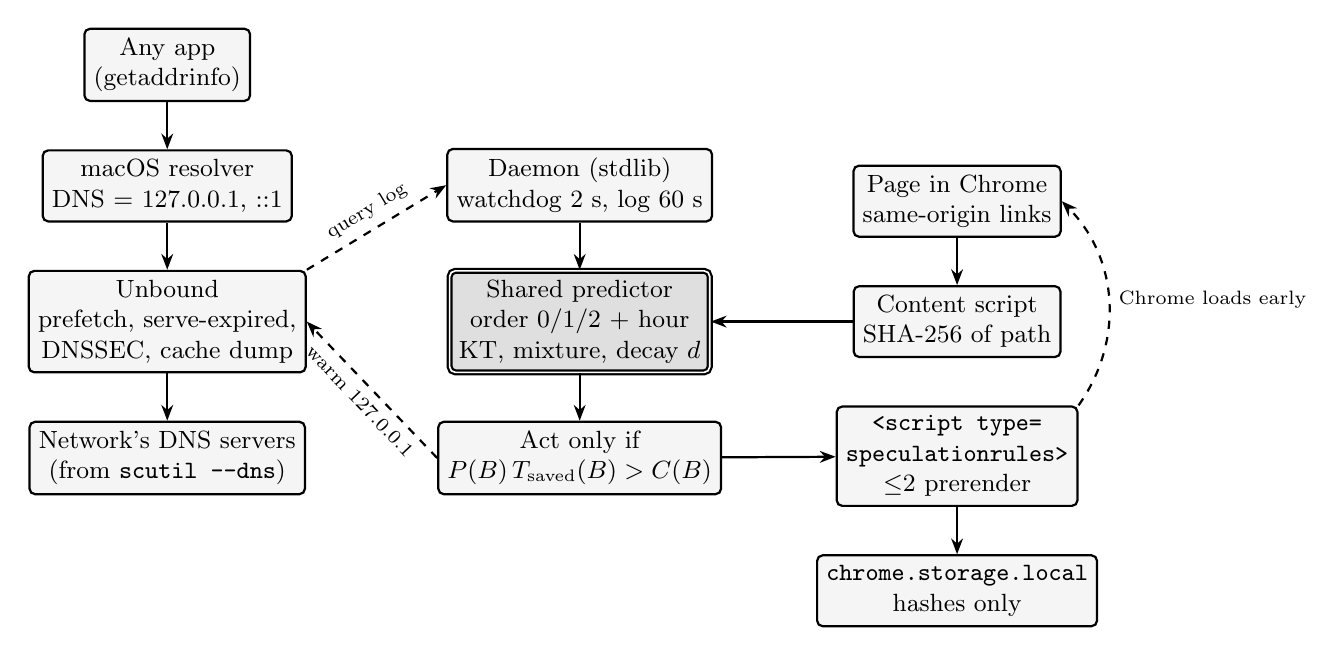
\begin{tikzpicture}[font=\small, node distance=6mm and 9mm,
  box/.style={draw, thick, rounded corners=2pt, align=center, minimum height=9mm, fill=gray!8},
  shared/.style={draw, thick, double, rounded corners=2pt, align=center, minimum height=9mm, fill=gray!25},
  arr/.style={-{Stealth[length=2mm]}, thick}, darr/.style={-{Stealth[length=2mm]}, thick, dashed}]
  % macOS column
  \node[box] (apps) {Any app\\(getaddrinfo)};
  \node[box, below=of apps] (mdns) {macOS resolver\\DNS = 127.0.0.1, ::1};
  \node[box, below=of mdns] (unb) {Unbound\\prefetch, serve-expired,\\DNSSEC, cache dump};
  \node[box, below=of unb] (up) {Network's DNS servers\\(from \texttt{scutil --dns})};
  \node[shared, right=18mm of unb] (pred) {Shared predictor\\order 0/1/2 + hour\\KT, mixture, decay $d$};
  \node[box, above=of pred] (daemon) {Daemon (stdlib)\\watchdog 2 s, log 60 s};
  \node[box, below=of pred] (rule) {Act only if\\$P(B)\,T_{\mathrm{saved}}(B) > C(B)$};
  \draw[arr] (apps) -- (mdns);
  \draw[arr] (mdns) -- (unb);
  \draw[arr] (unb) -- (up);
  \draw[darr] (unb.north east) -- node[above, sloped, font=\scriptsize]{query log} (daemon.west);
  \draw[arr] (daemon) -- (pred);
  \draw[arr] (pred) -- (rule);
  \draw[darr] (rule.west) -- node[below, sloped, font=\scriptsize]{warm 127.0.0.1} (unb.east);
  % Chrome column
  \node[box, right=18mm of pred] (cs) {Content script\\SHA-256 of path};
  \node[box, above=of cs] (page) {Page in Chrome\\same-origin links};
  \node[box, below=of cs] (rules) {\texttt{<script type=}\\\texttt{speculationrules>}\\$\le$2 prerender};
  \node[box, below=of rules] (store) {\texttt{chrome.storage.local}\\hashes only};
  \draw[arr] (page) -- (cs);
  \draw[arr] (cs) -- (pred);
  \draw[arr] (rule) -- (rules);
  \draw[arr] (rules) -- node[right, font=\scriptsize]{} (store);
  \draw[darr] (rules.north east) to[bend right=40] node[right, font=\scriptsize]{Chrome loads early} (page.east);
\end{tikzpicture}}

\newcommand{\timelinediagram}{%
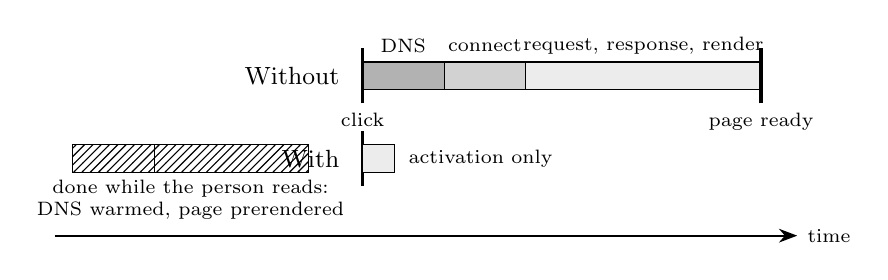
\begin{tikzpicture}[font=\small, x=1.15cm, y=7mm,
  seg/.style={draw, thick, minimum height=5mm, inner sep=0pt}]
  \foreach \y/\lab in {3/Without, 1.5/With} \node[anchor=east] at (-0.15, \y) {\lab};
  % without
  \draw[fill=gray!60] (0,2.75) rectangle (0.9,3.25); \node[font=\scriptsize] at (0.45,3.55) {DNS};
  \draw[fill=gray!35] (0.9,2.75) rectangle (1.8,3.25); \node[font=\scriptsize] at (1.35,3.55) {connect};
  \draw[fill=gray!15] (1.8,2.75) rectangle (4.4,3.25); \node[font=\scriptsize] at (3.1,3.55) {request, response, render};
  \draw[very thick] (0,2.5) -- (0,3.5); \node[font=\scriptsize, anchor=north] at (0,2.5) {click};
  \draw[very thick] (4.4,2.5) -- (4.4,3.5); \node[font=\scriptsize, anchor=north] at (4.4,2.5) {page ready};
  % with
  \draw[pattern=north east lines] (-3.2,1.25) rectangle (-2.3,1.75);
  \draw[pattern=north east lines] (-2.3,1.25) rectangle (-0.6,1.75);
  \node[font=\scriptsize, align=center] at (-1.9,0.75) {done while the person reads:\\DNS warmed, page prerendered};
  \draw[very thick] (0,1.0) -- (0,2.0); \draw[fill=gray!15] (0,1.25) rectangle (0.35,1.75);
  \node[font=\scriptsize, anchor=west] at (0.4,1.5) {activation only};
  \draw[-{Stealth}, thick] (-3.4,0.1) -- (4.8,0.1) node[right, font=\scriptsize] {time};
\end{tikzpicture}}

\newcommand{\C}[1]{\ifcsname c@#1\endcsname\csname c@#1\endcsname\else\textbf{??}\errmessage{missing confirm value #1}\fi}
\newcommand{\V}[1]{\ifcsname v@#1\endcsname\csname v@#1\endcsname\else\textbf{??}\errmessage{missing value #1}\fi}

\title{Predictive Loading: Learning a Person's Next DNS Lookup and Page Load\\from Their Own History}
\author{Reed Ostrov\\Denison University}
\date{November 2026}

\begin{document}
\maketitle

\begin{abstract}
People load the same names and pages in patterns. This paper predicts each person's next DNS lookup on macOS and next same-site page in Chrome from their own history, and does the waiting early when the expected time saved exceeds the measured cost. One predictor, a Bayesian mixture of order-0, order-1, order-2 and hour-of-day models with Krichevsky--Trofimov estimates and a daily-tuned decay, runs identically in Python and JavaScript. In offline replay of \V{r0.ntraces} traces it had lower log-loss than an order-1 Markov baseline on all \V{r0.wins_markov_bits}, and lower than PPM-C on \V{r0.wins_ppmc_bits}. On a campus network, API calls in later rounds were \V{r3.warm.paired}\,ms faster per call [\V{r3.warm.paired.lo}, \V{r3.warm.paired.hi}], first calls were \V{r3.cold.paired}\,ms slower, and the shared campus resolver beat a local resolver on median lookup time. The Chrome extension holds only the \texttt{storage} permission, stores only hashes, and never preloads action links.

\end{abstract}

\section{Introduction}
Most of the delay in opening a web page is waiting: for a name to resolve, for a connection, for the first byte. Much of that waiting is predictable. People return to the same sites, follow the same paths through them, and do so at similar times of day. If the next load can be guessed, the waiting can happen before the click.

This paper applies one idea at the two layers where speculative work is safe to do from the client: (1) DNS lookups for every application on macOS, where a wrong guess costs one cached query, and (2) full page loads inside Chrome, where the browser's Speculation Rules API \cite{specrules} can prefetch or prerender a same-origin page. Both layers use the same predictor, specified once and ported to Python and JavaScript; a test feeds both ports a 10{,}000-event sequence and requires byte-identical output.

The predictor is a Bayesian mixture of four context models (order 0, 1 and 2, and hour of day), each using the Krichevsky--Trofimov estimator \cite{kt1981} with an escape symbol. It acts on a candidate $B$ only when $P(B)\,T_{\mathrm{saved}}(B) > C(B)$, with both sides measured on the device. All data stays on the device; the Chrome extension stores only SHA-256 hashes of paths and holds the single permission \texttt{storage}.

Contributions: (i) a small, auditable predictor with a cost-aware decision rule that runs identically in two languages; (ii) a macOS resolver setup with watchdog, captive-portal, VPN and uninstall safety, tested by simulation; (iii) a Manifest V3 extension with no network access of its own; (iv) an evaluation that runs the offline kill test first, then measures lookup time, page loads at three Wi-Fi profiles, and API calls, against named baselines, reporting losses.

\section{Background}
\textbf{DNS caching.} A stub resolver asks a recursive resolver, which caches answers for their time to live (TTL). Unbound \cite{unbound} adds \emph{prefetch}, which refreshes a popular record shortly before it expires, and \emph{serve-expired}, which answers from an expired record when the upstream answer is slow (here after 400\,ms). Both help names already asked for recently. Neither helps a name that has dropped out of the cache or was never asked for on this network.

\textbf{Speculative page loading.} Chrome's Speculation Rules API lets a page list URLs to \emph{prefetch} (fetch the document) or \emph{prerender} (load and render it in a hidden tab, then swap it in on navigation). Eagerness settings control when: \texttt{immediate} at once, \texttt{moderate} on hover. instant.page \cite{instantpage} preloads on hover; Quicklink \cite{quicklink} prefetches links in the viewport when the browser is idle; Guess.js \cite{guessjs} uses site-wide analytics to predict the next page. None of these learns from the individual person.

\textbf{Sequence prediction.} Prediction by partial matching (PPM) \cite{cleary1984,moffat1990} blends context models of several orders through escape probabilities. Vitter and Krishnan \cite{vitter1996} showed that a good compressor is a good prefetcher. Padmanabhan and Mogul \cite{padmanabhan1996} measured predictive prefetching of web pages from server logs.

\section{Method}
\subsection{Events}
On the Mac, an event is a domain name in lookup order, read from Unbound's reply log. In Chrome, an event is the SHA-256 hash of a same-origin page path, with the query string and fragment dropped, kept per origin (itself hashed). A repeat of the previous event is ignored, so reloads count once.

\subsection{Context models and estimator}
Four models predict the next event $x$ from contexts $c$: the empty context (order 0), the previous event (order 1), the previous two events (order 2), and the local hour (0--23). In context $c$, with $k_c$ distinct symbols seen, repeat counts $n_x$ summing to $N_c$, and escape count $e_c$ (the number of times a symbol was new to $c$), the Krichevsky--Trofimov estimate over the $k_c$ symbols plus an escape symbol is
\[
P(x\mid c) = \frac{n_x + \tfrac12}{N_c + e_c + \tfrac12 (k_c+1)}, \qquad
P(\mathrm{esc}\mid c) = \frac{e_c + \tfrac12}{N_c + e_c + \tfrac12 (k_c+1)} .
\]
The escape mass goes to symbols not seen in $c$ in proportion to the order-0 model, and the order-0 escape is the probability of a brand-new event. Counts decay by a factor $d$ per event; storing counts scaled by $S=d^{-t}$ makes each update one addition, with renormalisation when $S>10^{100}$.

\subsection{Mixture and decay}
Model $i$ has weight $w_i \propto \prod_t P_i(x_t)^{d^{\,T-t}}$, kept as $\log w_i \leftarrow d\log w_i + \log P_i(x_t)$. The mixture is $P(x)=\sum_i w_i P_i(x)$. Six copies run in parallel with $d\in\{0.9, 0.95, 0.98, 0.99, 0.995, 0.999\}$; at each new day the copy with the lowest log-loss over the last 7 days is used. The previous event is never a candidate. Predictability is reported as bits per event, $-\frac1T\sum_t \log_2 P(x_t)$.

\subsection{Decision rule}
A candidate $B$ is acted on only if $P(B)\,T_{\mathrm{saved}}(B) > C(B)$. On the Mac, $T_{\mathrm{saved}}(B)$ is $B$'s measured upstream lookup time (an exponential average of uncached replies) and $C(B)$ is the measured time of a local query. In Chrome, $T_{\mathrm{saved}}(B)$ is $B$'s measured load time and $C(B)$ is the expected wasted bytes, $(1-P(B))$ times the page's measured size, divided by measured throughput. Prerender is chosen over prefetch only when its expected net gain is higher: prefetch saves only the network share of the load but wastes only the document; prerender saves the whole load but wastes the page with its subresources (estimated at four times the document). At most two prerenders are issued; other safe same-origin links get \texttt{moderate} (hover) prefetch.

\subsection{Measuring benefit}
Both tools keep a random holdout: 10\% of the Mac daemon's prefetch decisions and 20\% of the extension's top prediction are recorded but not acted on. Time saved is the holdout mean minus the treated mean, times treated hits, with a bootstrap interval and $n$; \texttt{predictive-loading stats} and the extension popup print these.

\begin{figure}[t]
\centering
\resizebox{\textwidth}{!}{\systemdiagram}
\caption{System. Left: every macOS app resolves through a local Unbound; the daemon reads its query log, predicts, and warms names through 127.0.0.1. Right: the extension's content script hashes the page path, predicts, and writes Speculation Rules. Both use the same predictor (double border).}
\label{fig:system}
\end{figure}

\section{Safety design}
\textbf{macOS.} Unbound listens only on 127.0.0.1 and ::1 and refuses all other clients; it validates DNSSEC, minimises query names, and hides its identity and version. It forwards to the resolvers the current network provides (\texttt{scutil --dns}). Both Unbound and the daemon run under launchd with KeepAlive. A watchdog asks Unbound for \texttt{localhost} every 2\,s and restores the original DNS settings after 3 failures. After any network change or wake, the Mac uses its original DNS (pass-through) until \texttt{captive.apple.com} returns its success page, so captive portals work; Apple's captive-portal names are forwarded uncached and never prefetched. When a VPN interface is up the tool steps aside fully. After a macOS or Unbound version change the daemon re-runs a health check (local answer, real lookup, and a SERVFAIL for \texttt{dnssec-failed.org}). The cache is dumped every 60\,s and at shutdown and reloaded at start. The daemon uses only the Python standard library, queries only 127.0.0.1, and writes data files with mode 600. Uninstall restores each network service's saved DNS list exactly and deletes every file.

\textbf{Chrome.} The extension requests only \texttt{storage}, has a strict content security policy, is not allowed in Incognito, and contains no \texttt{fetch}, \texttt{XMLHttpRequest}, WebSocket, \texttt{sendBeacon}, \texttt{eval}, \texttt{Function} or \texttt{innerHTML}. It writes speculation rules only for same-origin http(s) links, never for links whose path or text matches logout, sign-out, delete, remove, unsubscribe, cart, checkout, buy, pay, order, confirm, cancel or settings, never for downloads, and nothing when Data Saver is on. The link checks are adapted from instant.page (MIT) and Quicklink (Apache-2.0).

\begin{figure}[t]
\centering
\timelinediagram
\caption{Load timeline. Without prediction, DNS, connection and loading follow the click. With prediction, DNS is warmed and the page prerendered before the click, leaving only activation.}
\label{fig:timeline}
\end{figure}

\section{Experiments}
All timing experiments run on one MacBook (Apple silicon, macOS 26) on a campus Wi-Fi network. Root access is not used: Unbound runs on a high local port and the daemon runs unchanged against it. Network conditions are set by a local SOCKS5 proxy that adds a fixed round-trip delay per connection (10, 60 or 150\,ms, standing for home, busy campus and poor Wi-Fi) and resolves names either with the system resolver (Mac tool off) or through the local Unbound plus predictor (Mac tool on). Chrome is Chrome for Testing 159 driven by Playwright, with all host resolution forced through the proxy. Condition order is randomised per site or per round, medians and 75th percentiles are reported with bootstrap 95\% intervals (2{,}000 resamples), and $n$ is stated for every cell. Every number in this paper is read by a script from \texttt{RESULTS.md}, which is itself generated from the raw result files.

\textbf{Route 0, offline replay (kill test).} The predictor and four baselines (most popular, last successor, order-1 Markov with the same estimator, and PPM-C) replay public traces: MSNBC page categories, the NASA (July 1995) and ClarkNet (August 1995) HTTP logs, and Wikispeedia navigation paths, 1{,}000 users each, plus one recorded person's Chrome history (domains, and hashed paths per origin). Before running, the pass threshold was set: the mixture's log-loss must beat order-1 Markov with a 95\% interval below zero on most traces. The 30 users used for development were excluded.

\textbf{Route 1, lookups.} dnspyre resolves the Tranco top \V{r1.names} names, \V{r1.rounds} rounds \V{r1.wait}\,s apart, under three conditions: the network's resolver, Unbound alone with its own prefetch, and Unbound with the predictor's daemon.

\textbf{Route 2, page loads.} For each of 50 Tranco sites with a same-origin link that does not redirect, a session loads the home page, waits 1.5\,s (the time a person spends reading; the extension decides here), clicks the link, and records how long the person waited for the next page (load end minus prerender activation). Each session first visits home and the link once per DNS mode, so the extension has seen the path. The design is $2\times2$ (Mac tool, extension) at three Wi-Fi profiles; the six profile-by-extension sessions run at once, each with its own browser profile and proxy, and DNS mode order is shuffled per site.

\textbf{Route 3, API calls.} curl fetches one URL from each of \V{r3.hosts} API hosts, \V{r3.rounds} rounds, with the Mac tool off and on in shuffled order.

\section{Results}
\textbf{Route 0 passed.} The mixture's log-loss was lower than order-1 Markov's on \V{r0.wins_markov_bits} of \V{r0.ntraces} traces with the whole 95\% interval below zero, and lower than PPM-C's on \V{r0.wins_ppmc_bits} of \V{r0.ntraces} (Figure~\ref{fig:r0}). On NASA it used \V{r0.nasa_jul95.mixture.bits} bits per event against \V{r0.nasa_jul95.markov1.bits} for Markov-1 and \V{r0.nasa_jul95.ppm_c.bits} for PPM-C. On the recorded Chrome history it guessed the next domain first \V{r0.recorded_chrome_domains.mixture.top1}\% of the time (Markov-1 \V{r0.recorded_chrome_domains.markov1.top1}\%, PPM-C \V{r0.recorded_chrome_domains.ppm_c.top1}\%) and the next path within a site \V{r0.recorded_chrome_paths_per_origin.mixture.top1}\% of the time. Top-1 accuracy is low on the server logs (\V{r0.nasa_jul95.mixture.top1}\% on NASA) because most of their events are first visits.

\begin{figure}[t]
\centering
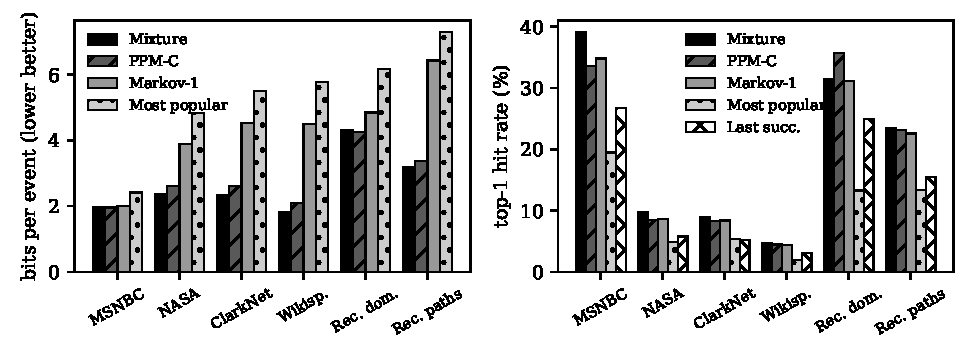
\includegraphics[width=\textwidth]{fig_route0.pdf}
\caption{Route 0, offline replay. Left: log-loss in bits per event. Right: share of events the method ranked first.}
\label{fig:r0}
\end{figure}

\textbf{Route 1.} On the first round, when nothing was cached, Unbound needed a median of \V{r1.cold.unbound_alone.median_ms}\,ms and Unbound with the predictor \V{r1.cold.unbound_plus_predictor.median_ms}\,ms, against \V{r1.cold.system_default.median_ms}\,ms for the campus resolver, which already held most popular names. In later rounds the medians were \V{r1.warm.system_default.median_ms}, \V{r1.warm.unbound_alone.median_ms} and \V{r1.warm.unbound_plus_predictor.median_ms}\,ms; at the 75th percentile, where expired records show, the predictor cut Unbound's \V{r1.warm.unbound_alone.p75_ms}\,ms to \V{r1.warm.unbound_plus_predictor.p75_ms}\,ms [\V{r1.warm.unbound_plus_predictor.p75_ci95.lo}, \V{r1.warm.unbound_plus_predictor.p75_ci95.hi}], but the shared campus resolver stayed fastest at \V{r1.warm.system_default.p75_ms}\,ms (Figure~\ref{fig:r1}).

\begin{figure}[t]
\centering
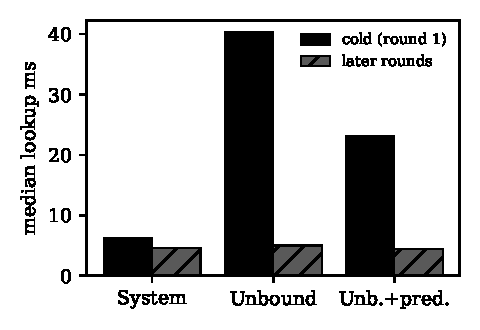
\includegraphics[width=0.55\textwidth]{fig_route1.pdf}
\caption{Route 1, median lookup time for the Tranco top \V{r1.names}.}
\label{fig:r1}
\end{figure}

\textbf{Route 2.} Table~\ref{tab:r2} and Figure~\ref{fig:r2} give the medians for \V{r2.n} measured visits (\V{r2.errors} site failures excluded). The paired extension effect on the wait for the next page was \V{r2.10.eff.ext}\,ms [\V{r2.10.eff.ext.lo}, \V{r2.10.eff.ext.hi}] at 10\,ms, \V{r2.60.eff.ext}\,ms [\V{r2.60.eff.ext.lo}, \V{r2.60.eff.ext.hi}] at 60\,ms and \V{r2.150.eff.ext}\,ms [\V{r2.150.eff.ext.lo}, \V{r2.150.eff.ext.hi}] at 150\,ms (negative is faster). The Mac tool's paired effect on the home page load was \V{r2.10.eff.mac}, \V{r2.60.eff.mac} and \V{r2.150.eff.mac}\,ms at the three profiles.

\begin{table}[t]
\centering\small
\begin{tabular}{lrrrr}
\toprule
 & \multicolumn{2}{c}{Extension off} & \multicolumn{2}{c}{Extension on}\\
Wi-Fi profile & Mac off & Mac on & Mac off & Mac on\\
\midrule
Home, 10 ms & \V{r2.10.off.off.next} & \V{r2.10.off.on.next} & \V{r2.10.on.off.next} & \V{r2.10.on.on.next}\\
Campus, 60 ms & \V{r2.60.off.off.next} & \V{r2.60.off.on.next} & \V{r2.60.on.off.next} & \V{r2.60.on.on.next}\\
Poor, 150 ms & \V{r2.150.off.off.next} & \V{r2.150.off.on.next} & \V{r2.150.on.off.next} & \V{r2.150.on.on.next}\\
\bottomrule
\end{tabular}
\caption{Route 2, median wait for the next page (ms).}
\label{tab:r2}
\end{table}

\begin{figure}[t]
\centering
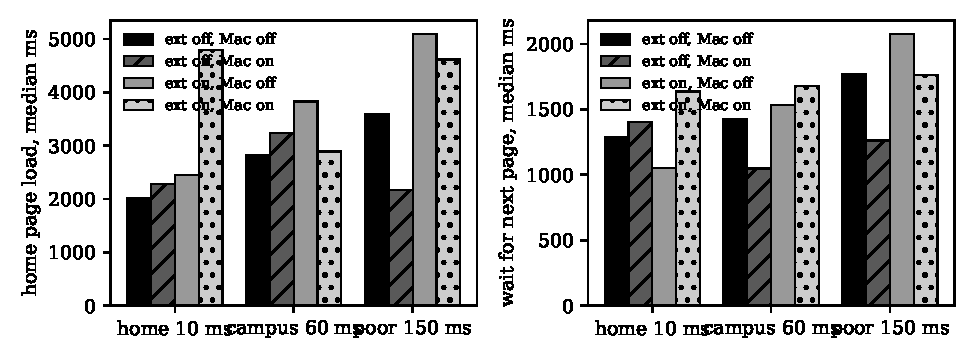
\includegraphics[width=\textwidth]{fig_route2.pdf}
\caption{Route 2 by Wi-Fi profile. Left: home page load. Right: wait for the next page after the click.}
\label{fig:r2}
\end{figure}

\textbf{Route 3.} For API calls in later rounds the Mac tool saved a paired median of \V{r3.warm.paired}\,ms [\V{r3.warm.paired.lo}, \V{r3.warm.paired.hi}] per call ($n=\V{r3.warm.paired.n}$; median total \V{r3.warm.off.total} vs \V{r3.warm.on.total}\,ms). On the first round it cost \V{r3.cold.paired}\,ms [\V{r3.cold.paired.lo}, \V{r3.cold.paired.hi}] ($n=\V{r3.cold.paired.n}$), because a cold local Unbound resolves from the root down while the campus resolver already holds the names.

\section{Benchmarks}
\textbf{Prediction.} Against the four predictors, the mixture had the lowest log-loss on most traces. It lost to PPM-C on bits for the recorded domains (\V{r0.recorded_chrome_domains.mixture.bits} vs \V{r0.recorded_chrome_domains.ppm_c.bits}) and MSNBC (\V{r0.msnbc.mixture.bits} vs \V{r0.msnbc.ppm_c.bits}), and on top-1 for the recorded domains (\V{r0.recorded_chrome_domains.mixture.top1}\% vs \V{r0.recorded_chrome_domains.ppm_c.top1}\%).

\textbf{Pages.} At 60\,ms, with a person who hovers 300\,ms before clicking, the median wait for the next page was \V{pb.default.med}\,ms with Chrome's default ($n=\V{pb.default.n}$), \V{pb.instantpage.med}\,ms with instant.page ($n=\V{pb.instantpage.n}$), \V{pb.quicklink.med}\,ms with Quicklink ($n=\V{pb.quicklink.n}$) and \V{pb.extension.med}\,ms with this extension ($n=\V{pb.extension.n}$). Quicklink made \V{pb.quicklink.spec} speculative requests to serve its hits; the extension made \V{pb.extension.spec}. This benchmark covers only the sites finished in the time available, so its intervals are wide (see \texttt{RESULTS.md}).

\textbf{Lookups.} Against plain Unbound, the predictor lowered both the cold median and the warm 75th percentile (Route 1). Against the network's own resolver it did not: a shared campus resolver serves popular names from a cache filled by thousands of users.

\section{Limitations}
All timing comes from one Mac on one campus network over one evening; a home network with a slow or distant resolver would favour the Mac tool more, and the campus result likely understates it. Route 2's training is one visit per site, far less history than a person builds, and its sites are the most popular on the web. The Safari arm of Route 2, the live check on the author's own Mac and Chrome, and installation with real port-53 DNS settings need an administrator password and were not run unattended; the macOS safety behaviours were tested with real Unbound and simulated system tools. The page benchmark's $n$ is small. The extension's last-write-wins storage can lose an update when two tabs of one site navigate at the same instant.

\section{Confirmatory experiments}
\label{sec:confirm}
The experiments in Section~\ref{sec:results} were designed before any data existed but were not pre-registered, and one of them (Route~1) has a design flaw described below. This section reports three further experiments whose hypotheses, primary metrics, statistics and exclusion rules were committed to the public repository (\texttt{PREREG.md}, commit \texttt{f830fdd}, 02:38 EST on 20 November 2026) together with the analysis script, before any of their data was collected. The analysis was run once.

\subsection{Statistics}
Every primary comparison is paired. For a set of paired differences $d_1,\dots,d_n$ (treatment minus control, so negative means faster) we report the Hodges--Lehmann estimate, the median of all Walsh averages $(d_i+d_j)/2$, $i\le j$, which is robust to the heavy right tail of network timings; a 95\% percentile bootstrap interval over pairs (10{,}000 resamples, fixed seed); and a two-sided Wilcoxon signed-rank $p$-value. The three paired primary tests are Holm-corrected as a family. A unit (host-round, test day, site) with any failed measurement in either arm is dropped from both arms; dropped counts are reported. Nothing was stopped early or rerun.

\subsection{E1: live replication on the current network}
E1 reruns Routes~1 and 3 on Denison campus Wi-Fi, whose DHCP resolver is a shared campus resolver. Because the Mac tool was live on the test machine, the benchmark harness was changed to send its ``network resolver'' arm directly to the DHCP resolver instead of through the system resolver, which by then pointed at the local Unbound. \emph{Disclosure:} E1 started before the pre-registration was written, and per-round medians of its first two rounds had been printed and seen. E1 is therefore a replication with a fixed analysis, not a blind test.

\emph{Design flaw in Route~1.} Name order is shuffled each round, but the same 500 names repeat every 180\,s, which is shorter than many of their TTLs. ``Warm'' rounds therefore mostly measure how long each arm keeps answers cached, and the predictor arm benefits from repeatedly re-fetching a small fixed set. Route~1 and E1a are upper bounds for an unrealistically repetitive workload; E2 is the test that removes this flaw. The E1a script keeps only per-arm summaries, so E1a is reported as unpaired medians and is outside the Holm family. E1b (50 API hosts, 5 rounds, 120\,s apart, host and mode order shuffled) keeps every request and is analysed paired by host and round, using rounds 2--5.

\subsection{E2: trace-driven simulation on held-out real history}
\emph{Workload.} One person's Chrome history: \C{e2.events_total} page visits to \C{e2.names} distinct host names over 11 weeks, with real timestamps, read in memory only. Each visit is one lookup of its host. Subresource lookups (images, scripts, third-party hosts) are not in the history and are not modelled.

\emph{Split.} Chronological. The predictor learns online from the first visit; only the last 14 days (\C{e2.events_test_simulated} lookups) are scored. No parameter was tuned on the test days.

\emph{Measured inputs.} For each name, the full TTL was taken from the first answer of a freshly started, fully recursive local Unbound with an empty cache (minimum TTL along any CNAME chain), and the network latency as the median of 3 queries to the campus resolver. \C{e2.names_measured} of \C{e2.names} names answered both. A local cache hit costs the measured median time of a cached query to the live local Unbound, \C{e2.local_hit_ms}\,ms.

\emph{Policies.} (S) a plain TTL cache, as macOS keeps; (U) S plus Unbound's prefetch, which refreshes a name queried in the last 10\% of its TTL; (P) U plus the shipped predictor and cost rule, run every 60\,s of trace time while the machine is awake (an awake gap is a gap under 30 minutes between visits), with the daemon's one-hour pending rule and its next-hour look-ahead on wake. The shipped 10\% holdout is off in the simulation. A miss costs the name's measured network latency. Each policy's upstream queries in the test period are counted as its cost.

\emph{Primary metric.} Per test day, mean lookup latency; paired difference P minus S over the 14 days.

\subsection{E3: the Chrome extension under a habit}
Route~2 gave each site one training visit, far less history than a person builds, so the extension rarely passed its own cost rule. E3 tests the condition the extension is built for: a person who repeatedly takes the same path.

\emph{Design.} The 50 sites of Route~2, each with a home page and one same-site next page. For each site and arm (extension on or off, order random per site), a fresh browser profile runs 8 training visits (load home, read 3\,s, click the next link) and then 6 measured visits. Before each measured visit the proxy drops all connections; the HTTP cache is kept, as a habitual visitor's would be. Chrome for Testing runs through the bench SOCKS proxy with 60\,ms added round-trip time and the campus resolver for DNS in both arms. Four sites run in parallel, each with its own proxy. The extension's 20\% holdout stays on, so the estimate is intention-to-treat: what a user gets from the shipped extension, including the 1 in 5 confident predictions it deliberately does not act on.

\emph{Primary metric.} Per site, the median next-page wait (\texttt{loadEventEnd} minus \texttt{activationStart}) over the 6 measured visits; paired difference on minus off over sites. With 50 pairs the Wilcoxon test has 80\% power at $\alpha=0.05$ for a standardised paired effect of about 0.41. Secondary: the share of measured next pages served preloaded, and the home-page load difference (the extension's own overhead).

\subsection{Results}
Deviations from the pre-registration, all logged in \texttt{results/rerun-2026-11-20/deviations.txt}: (i) the repository test suite (about 2 minutes, mostly local CPU) ran on the same machine during E1b; (ii) the disk filled as E1b finished, so the step that copies its output failed and was redone by hand from the same files; no measurement was lost; (iii) E2's 14-day test window spans \C{e2.test_days} calendar days, so the per-day analysis has \C{e2.primary_P_minus_S_per_day.n} pairs, not 14.

\textbf{E1a (live DNS, unpaired, outside the Holm family).} Median lookup time, round 1 (cold) and rounds 2--5 (warm), with 95\% bootstrap intervals:
\begin{center}\small
\begin{tabular}{@{}lrr@{}}
\toprule
Arm & Cold median (ms) & Warm median (ms) \\
\midrule
Campus resolver (direct) & \C{e1a.cold.system_default.median_ms} [\C{e1a.cold.system_default.median_ci95.lo}, \C{e1a.cold.system_default.median_ci95.hi}] & \C{e1a.warm.system_default.median_ms} [\C{e1a.warm.system_default.median_ci95.lo}, \C{e1a.warm.system_default.median_ci95.hi}] \\
Unbound alone & \C{e1a.cold.unbound_alone.median_ms} [\C{e1a.cold.unbound_alone.median_ci95.lo}, \C{e1a.cold.unbound_alone.median_ci95.hi}] & \C{e1a.warm.unbound_alone.median_ms} [\C{e1a.warm.unbound_alone.median_ci95.lo}, \C{e1a.warm.unbound_alone.median_ci95.hi}] \\
Unbound + predictor & \C{e1a.cold.unbound_plus_predictor.median_ms} [\C{e1a.cold.unbound_plus_predictor.median_ci95.lo}, \C{e1a.cold.unbound_plus_predictor.median_ci95.hi}] & \C{e1a.warm.unbound_plus_predictor.median_ms} [\C{e1a.warm.unbound_plus_predictor.median_ci95.lo}, \C{e1a.warm.unbound_plus_predictor.median_ci95.hi}] \\
\bottomrule
\end{tabular}
\end{center}
The predictor made the local resolver faster than Unbound alone, but on this network the shared campus resolver, kept warm by thousands of users, was faster than either local arm in both phases. A local resolver adds a full recursion path (Unbound forwards to the campus resolver, which is already the fast path), so on a network with a fast, busy shared resolver the Mac tool adds latency it cannot recover by prediction alone.

\textbf{E1b (live API calls, paired).} Over \C{e1b.warm.n} host-round pairs in rounds 2--5 (\C{e1b.dropped_units} units dropped), the Hodges--Lehmann estimate of total request time with the Mac tool on minus off was \C{e1b.warm.hl}\,ms [\C{e1b.warm.ci.lo}, \C{e1b.warm.ci.hi}], Wilcoxon $p=\C{e1b.warm.p}$ (Holm $p=\C{holm.e1b}$), against an off-arm median request of \C{e1b.off_median_ms}\,ms. First-round calls: \C{e1b.cold.hl}\,ms [\C{e1b.cold.ci.lo}, \C{e1b.cold.ci.hi}].

\textbf{E2 (held-out real history).} Over \C{e2.events_test_simulated} test-period lookups (\C{e2.names_measured} measured names; median TTL \C{e2.ttl_median_s}\,s; median campus-resolver latency \C{e2.net_ms_median}\,ms, 90th percentile \C{e2.net_ms_p90}\,ms):
\begin{center}\small
\begin{tabular}{@{}lrrr@{}}
\toprule
Policy & Cache hit rate & Mean lookup (ms) & Upstream queries per awake hour \\
\midrule
S: TTL cache only & \C{e2.hit_rate.S} & \C{e2.mean_ms.S} & \C{e2.upstream_per_awake_hour.S} \\
U: + Unbound prefetch & \C{e2.hit_rate.U} & \C{e2.mean_ms.U} & \C{e2.upstream_per_awake_hour.U} \\
P: + predictor & \C{e2.hit_rate.P} & \C{e2.mean_ms.P} & \C{e2.upstream_per_awake_hour.P} \\
\bottomrule
\end{tabular}
\end{center}
Primary: per day, P minus S was \C{e2.primary_P_minus_S_per_day.hl}\,ms per lookup [\C{e2.primary_P_minus_S_per_day.ci.lo}, \C{e2.primary_P_minus_S_per_day.ci.hi}], faster on every one of the \C{e2.primary_P_minus_S_per_day.n} days (Wilcoxon $p=\C{e2.primary_P_minus_S_per_day.p}$, Holm $p=\C{holm.e2}$). The predictor's own contribution over Unbound's prefetch (P minus U) was \C{e2.P_minus_U_per_day.hl}\,ms [\C{e2.P_minus_U_per_day.ci.lo}, \C{e2.P_minus_U_per_day.ci.hi}]. The effect is reliable and small: the predictor raises the hit rate by about 3.6 points, and each extra hit saves one network lookup of about 6\,ms on this network. The price is upstream traffic: P sends about 2.3 times as many queries per awake hour as S. Because a miss costs the network latency, the absolute saving scales with it (exploratory): at a 30\,ms home-router resolver the same hit-rate gain would save roughly 1\,ms per lookup, and at 100\,ms roughly 3.6\,ms.

\textbf{E3 (Chrome extension under a habit).} \E3RESULT


\section{Related work}
Padmanabhan and Mogul \cite{padmanabhan1996} predicted next requests from server-side access patterns and measured latency reduction against extra traffic, the same trade the decision rule here makes per candidate. Vitter and Krishnan \cite{vitter1996} proved that prefetchers built on universal compressors approach the optimal fault rate; the predictor here is such a compressor-style model, scored in bits per event. PPM \cite{cleary1984} and its escape method C \cite{moffat1990} are the classical way to blend contexts of several orders; this work instead mixes whole models by their decayed past performance and uses the KT estimator \cite{kt1981} inside each. Guess.js \cite{guessjs} predicts next pages from aggregate analytics on the server; here prediction is per person and never leaves the device. instant.page \cite{instantpage} and Quicklink \cite{quicklink} are history-free heuristics; the Speculation Rules API \cite{specrules} is the browser mechanism this work drives.

\section{Conclusion}
A per-person mixture predictor, gated by a measured cost-benefit rule, beats order-1 Markov prediction on every trace tested and can run safely at two layers: as a local resolver's prefetcher and as a Speculation Rules writer. The gains it delivers depend on what it replaces. Against a shared resolver on a fast campus network, local DNS warming saves little and costs time on first lookups; the page layer, which hides a whole load behind the time a person spends reading, is where the idea pays. The code, tests, data scripts and this paper's numbers are in the public repository.


\begin{thebibliography}{10}\small
\bibitem{padmanabhan1996} V.~N. Padmanabhan and J.~C. Mogul. Using predictive prefetching to improve World Wide Web latency. \emph{ACM SIGCOMM Computer Communication Review}, 26(3):22--36, 1996. doi:10.1145/235160.235164.
\bibitem{vitter1996} J.~S. Vitter and P.~Krishnan. Optimal prefetching via data compression. \emph{Journal of the ACM}, 43(5):771--793, 1996. doi:10.1145/234752.234753.
\bibitem{cleary1984} J.~G. Cleary and I.~H. Witten. Data compression using adaptive coding and partial string matching. \emph{IEEE Transactions on Communications}, 32(4):396--402, 1984. doi:10.1109/TCOM.1984.1096090.
\bibitem{moffat1990} A.~Moffat. Implementing the PPM data compression scheme. \emph{IEEE Transactions on Communications}, 38(11):1917--1921, 1990. doi:10.1109/26.61469.
\bibitem{kt1981} R.~E. Krichevsky and V.~K. Trofimov. The performance of universal encoding. \emph{IEEE Transactions on Information Theory}, 27(2):199--207, 1981. doi:10.1109/TIT.1981.1056331.
\bibitem{guessjs} Guess.js contributors. Guess.js: libraries and tools for enabling data-driven user experiences on the web. \url{https://github.com/guess-js/guess}, 2018--2026.
\bibitem{specrules} WICG. Speculation Rules. \url{https://wicg.github.io/nav-speculation/speculation-rules.html}, accessed November 2026.
\bibitem{instantpage} A.~Dieulot. instant.page. \url{https://instant.page/}, v5.2.0.
\bibitem{quicklink} Google Chrome Labs. Quicklink. \url{https://github.com/GoogleChromeLabs/quicklink}, v3.0.1.
\bibitem{unbound} NLnet Labs. Unbound DNS resolver. \url{https://nlnetlabs.nl/projects/unbound/}, v1.26.2.
\end{thebibliography}
\end{document}
